
\subsection{Descripción de los datos}
Con el objeto de que el lector pueda hacerse a una idea lo más completa posible sobre los requisitos de información del sistema y el planteamiento teórico de los datos utilizados, se expone un diagrama UML entidad-relación. Este tipo de diagrama muestra el funcionamiento de la base de datos a nivel lógico, y suele servir como primera aproximación al desarrollo de la base de datos en la fase de diseño. Tiene 3 elementos principales:
\begin{enumerate}
	\item \textbf{Entidades:} Objetos o conceptos del dominio sobre los que se almacena información. Se representan mediante rectángulos.
	
	\item \textbf{Atributos:} Propiedades que describen a las entidades. Se representan mediante elipses conectadas a su entidad, y la clave primaria se suele subrayar.
	
	\item \textbf{Relaciones:} Asociaciones entre entidades que describen cómo se vinculan entre sí. Se representan mediante rombos y se caracterizan por su cardinalidad (1:1, 1:N o N:N). Existen relaciones específicas que identifican herencia, representadas por triángulos invertidos.
	
	\item \textbf{Cardinalidad:} Restricción que indica cuántas instancias de una entidad pueden participar en una relación con otra (uno a uno, uno a muchos o muchos a muchos).
\end{enumerate}

Adicionalmente, se mostrará un diccionario de datos. Un diccionario de datos es un documento que describe de forma estructurada la información que el sistema almacena y gestiona, detallando para cada elemento su nombre, su tipo de dato, sus restricciones y las relaciones que mantiene con el resto de elementos del modelo. En este apartado se presentan los campos que componen las entidades del sistema de forma genérica, con el propósito de que el lector pueda comprender la naturaleza y organización de la información tratada, sin que ello implique una correspondencia literal con la implementación final.

\subsubsection{Diagrama Entidad-Relación}

\begin{figure}[H]
	\centering
	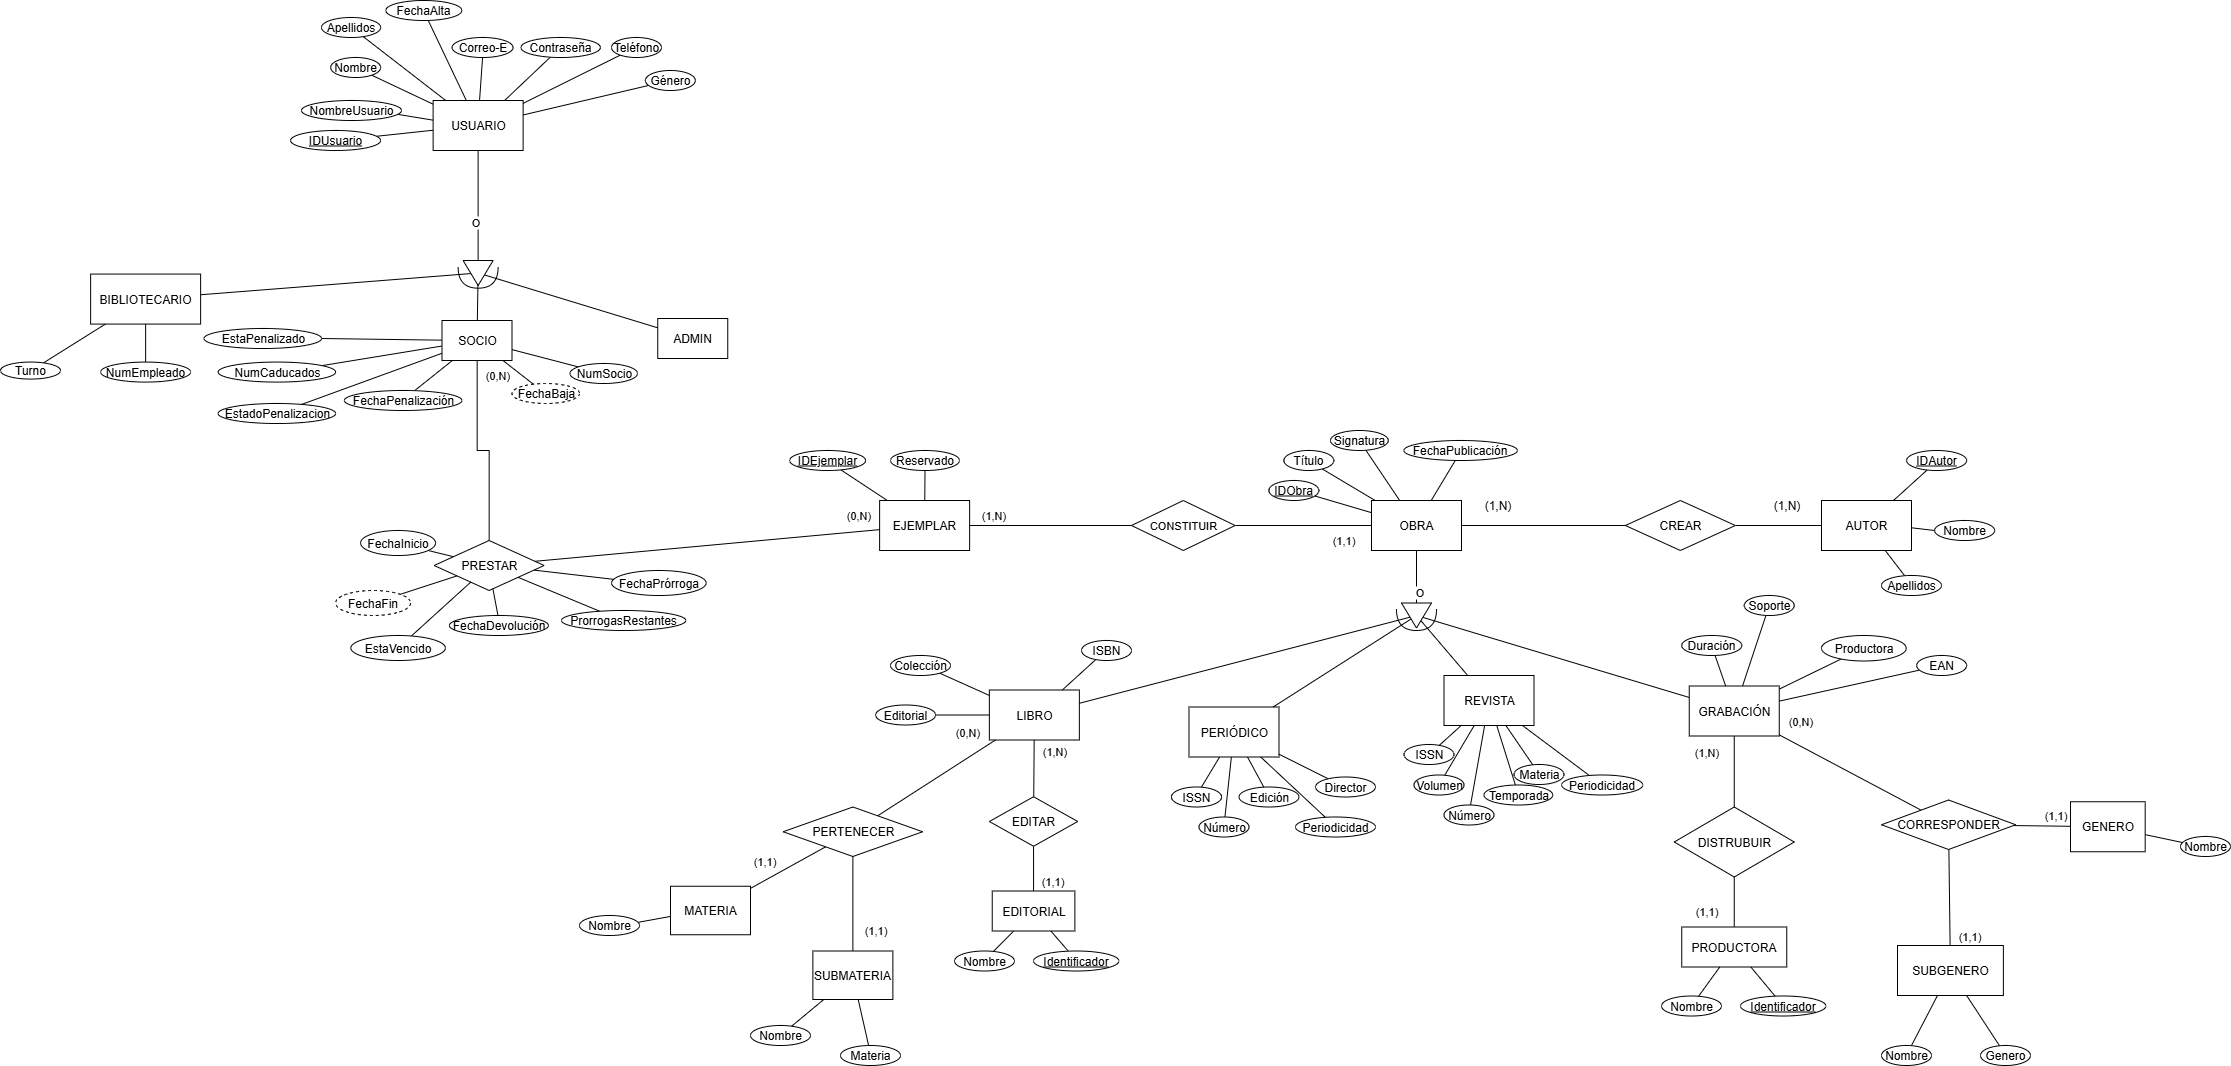
\includegraphics[width=\textwidth]{imagenes/diagrama_er.png}
	\caption{Diagrama entidad-relación de Liber.}
	\label{fig:diagrama_er}
\end{figure}

\subsection{Diccionario de datos}

A continuación se presenta el diccionario de datos del sistema, que recoge de forma estructurada las entidades y relaciones que lo componen, sus atributos, las restricciones que los rigen y las reglas específicas de cada campo. Se distinguen dos grandes bloques: por un lado, las entidades (los objetos del dominio con existencia propia) y, por otro, las relaciones (los vínculos entre dichas entidades).

\subsubsection*{Entidades}

\subsubsection{Entidad: AUTOR}
\begin{itemize}
	\item\textbf{Definición:} Representación de la persona que escribe una obra.
	\item\textbf{Reglas:} Un autor puede tener asociadas múltiples obras, pero no es obligatorio que tenga un apellido registrado (por ejemplo, en el caso de autores anónimos).
\end{itemize}

\begin{table}[H]
	\centering
	\caption{Atributos de la entidad AUTOR.}
	\label{tab:dict_autor}
	\small
	\begin{tabularx}{\textwidth}{l l X l c c X}
		\toprule
		\textbf{ID} & \textbf{Nombre} & \textbf{Definición} & \textbf{Tipo} & \textbf{Único} & \textbf{Nulo} & \textbf{Reglas} \\
		\midrule
		E01.1 & IDAutor & Identificador del autor en el sistema. & Número entero & Sí & No & Clave primaria, autoincremental. \\
		\addlinespace
		E01.2 & Nombre & Nombre del autor. & Texto (máx. 50) & No & No & -- \\
		\addlinespace
		E01.3 & Apellidos & Apellidos del autor. & Texto (máx. 255) & No & Sí & -- \\
		\bottomrule
	\end{tabularx}
\end{table}

\begin{itemize}
	\item\textbf{Identificador:} IDAutor (E01.1)
\end{itemize}

\subsubsection{Entidad: EDITORIAL}
\begin{itemize}
	\item\textbf{Definición:} Representación de las entidades encargadas de publicar y editar libros.
	\item\textbf{Reglas:} Una editorial puede tener múltiples libros asociados.
\end{itemize}

\begin{table}[H]
	\centering
	\caption{Atributos de la entidad EDITORIAL.}
	\label{tab:dict_editorial}
	\small
	\begin{tabularx}{\textwidth}{l l X l c c X}
		\toprule
		\textbf{ID} & \textbf{Nombre} & \textbf{Definición} & \textbf{Tipo} & \textbf{Único} & \textbf{Nulo} & \textbf{Reglas} \\
		\midrule
		E02.1 & Identificador & Identificador de la editorial en el sistema. & Número entero & Sí & No & Clave primaria, autoincremental. \\
		\addlinespace
		E02.2 & Nombre & Nombre comercial de la editorial. & Texto (máx. 50) & No & No & -- \\
		\bottomrule
	\end{tabularx}
\end{table}

\begin{itemize}
	\item\textbf{Identificador:} Identificador (E02.1)
\end{itemize}

\subsubsection{Entidad: EJEMPLAR}
\begin{itemize}
	\item\textbf{Definición:} Representación de cada ejemplar físico dentro de la biblioteca.
	\item\textbf{Reglas:} Cada ejemplar debe estar asociado a una obra preexistente. El estado (disponible o prestado) no se almacena, sino que se calcula a partir de la existencia de un préstamo activo.
\end{itemize}

\begin{table}[H]
	\centering
	\caption{Atributos de la entidad EJEMPLAR.}
	\label{tab:dict_ejemplar}
	\small
	\begin{tabularx}{\textwidth}{l l X l c c X}
		\toprule
		\textbf{ID} & \textbf{Nombre} & \textbf{Definición} & \textbf{Tipo} & \textbf{Único} & \textbf{Nulo} & \textbf{Reglas} \\
		\midrule
		E03.1 & IDEjemplar & Identificador del ejemplar. & Número entero & Sí & No & Clave primaria, autoincremental. \\
		\addlinespace
		E03.2 & IDObra & Referencia a la obra asociada. & Número entero & No & No & Clave foránea FK $\rightarrow$ OBRA (E06.1). \\
		\addlinespace
		E03.3 & Reservado & Indica si ha sido reservado. & Booleano & No & No & Valor por defecto: Falso (0). \\
		\bottomrule
	\end{tabularx}
\end{table}

\begin{itemize}
	\item\textbf{Identificador:} IDEjemplar (E03.1)
\end{itemize}

\subsubsection{Entidad: GÉNERO}
\begin{itemize}
	\item\textbf{Definición:} Clasificación temática general de las grabaciones.
	\item\textbf{Reglas:} El nombre del género debe ser único.
\end{itemize}

\begin{table}[H]
	\centering
	\caption{Atributos de la entidad GÉNERO.}
	\label{tab:dict_genero}
	\small
	\begin{tabularx}{\textwidth}{l l X l c c X}
		\toprule
		\textbf{ID} & \textbf{Nombre} & \textbf{Definición} & \textbf{Tipo} & \textbf{Único} & \textbf{Nulo} & \textbf{Reglas} \\
		\midrule
		E04.1 & Nombre & Nombre del género. & Texto (máx. 50) & Sí & No & Clave primaria natural. \\
		\bottomrule
	\end{tabularx}
\end{table}

\begin{itemize}
	\item\textbf{Identificador:} Nombre (E04.1)
\end{itemize}

\subsubsection{Entidad: LIBRO (Especialización de OBRA)}
\begin{itemize}
	\item\textbf{Definición:} Representación específica de un libro, heredando las propiedades de la Obra.
	\item\textbf{Reglas:} El ISBN debe ser único y la editorial es un campo obligatorio.
\end{itemize}

\begin{table}[H]
	\centering
	\caption{Atributos de la entidad LIBRO.}
	\label{tab:dict_libro}
	\small
	\begin{tabularx}{\textwidth}{l l X l c c X}
		\toprule
		\textbf{ID} & \textbf{Nombre} & \textbf{Definición} & \textbf{Tipo} & \textbf{Único} & \textbf{Nulo} & \textbf{Reglas} \\
		\midrule
		E11.1 & ISBN & Número Internacional Normalizado para Libros. & Texto (máx. 13) & Sí & No & Clave primaria. Formato ISBN-10 o ISBN-13. \\
		\addlinespace
		E11.2 & IDEditorial & Referencia a la editorial. & Número entero & No & No & Clave foránea FK $\rightarrow$ EDITORIAL (E02.1). \\
		\addlinespace
		E11.3 & IDMateria & Referencia a la materia principal. & Número entero & No & Sí & Clave foránea FK $\rightarrow$ MATERIA (E05.1). \\
		\addlinespace
		E11.4 & IDSubmateria & Referencia a la submateria. & Número entero & No & Sí & Clave foránea FK $\rightarrow$ SUBMATERIA (E09.1). \\
		\addlinespace
		E11.5 & Colección & Nombre de la colección. & Texto (máx. 255) & No & Sí & -- \\
		\bottomrule
	\end{tabularx}
\end{table}

\begin{itemize}
	\item\textbf{Identificador:} ISBN (E11.1)
\end{itemize}

\subsubsection{Entidad: MATERIA}
\begin{itemize}
	\item\textbf{Definición:} Área de conocimiento general que clasifica las obras.
	\item\textbf{Reglas:} El nombre de la materia debe ser único.
\end{itemize}

\begin{table}[H]
	\centering
	\caption{Atributos de la entidad MATERIA.}
	\label{tab:dict_materia}
	\small
	\begin{tabularx}{\textwidth}{l l X l c c X}
		\toprule
		\textbf{ID} & \textbf{Nombre} & \textbf{Definición} & \textbf{Tipo} & \textbf{Único} & \textbf{Nulo} & \textbf{Reglas} \\
		\midrule
		E05.1 & Nombre & Nombre de la materia. & Texto (máx. 50) & Sí & No & Clave primaria natural. \\
		\bottomrule
	\end{tabularx}
\end{table}

\begin{itemize}
	\item\textbf{Identificador:} Nombre (E05.1)
\end{itemize}

\subsubsection{Entidad: OBRA}
\begin{itemize}
	\item\textbf{Definición:} Representación conceptual de un título del catálogo, agrupando ejemplares y centralizando la relación con los autores.
	\item\textbf{Reglas:} La signatura debe ser única en todo el catálogo. El tipo de obra debe ser uno de los cuatro definidos.
\end{itemize}

\begin{table}[H]
	\centering
	\caption{Atributos de la entidad OBRA.}
	\label{tab:dict_obra}
	\small
	\begin{tabularx}{\textwidth}{l l X l c c X}
		\toprule
		\textbf{ID} & \textbf{Nombre} & \textbf{Definición} & \textbf{Tipo} & \textbf{Único} & \textbf{Nulo} & \textbf{Reglas} \\
		\midrule
		E06.1 & IDObra & Identificador de la obra. & Número entero & Sí & No & Clave primaria, autoincremental. \\
		\addlinespace
		E06.2 & Título & Título principal de la obra. & Texto (máx. 255) & No & No & -- \\
		\addlinespace
		E06.3 & Signatura & Código de localización. & Texto (máx. 50) & Sí & No & Código alfanumérico. \\
		\addlinespace
		E06.4 & FechaPublicación & Fecha de publicación original. & Fecha & No & Sí & Formato AAAA-MM-DD. \\
		\addlinespace
		E06.5 & Tipo & Categoría de la obra. & Lista de opciones & No & No & Valores: LIBRO, REVISTA, PERIODICO, GRABACION. \\
		\bottomrule
	\end{tabularx}
\end{table}

\begin{itemize}
	\item\textbf{Identificador:} IDObra (E06.1)
\end{itemize}

\subsubsection{Entidad: PERIÓDICO (Especialización de OBRA)}
\begin{itemize}
	\item\textbf{Definición:} Publicación seriada de frecuencia regular.
	\item\textbf{Reglas:} Hereda de Obra. Los periódicos no pueden prestarse.
\end{itemize}

\begin{table}[H]
	\centering
	\caption{Atributos de la entidad PERIÓDICO.}
	\label{tab:dict_periodico}
	\small
	\begin{tabularx}{\textwidth}{l l X l c c X}
		\toprule
		\textbf{ID} & \textbf{Nombre} & \textbf{Definición} & \textbf{Tipo} & \textbf{Único} & \textbf{Nulo} & \textbf{Reglas} \\
		\midrule
		E12.1 & ISSN & Número Internacional de Publicaciones Seriadas. & Texto (máx. 8) & Sí & No & Clave primaria. Formato ISSN. \\
		\addlinespace
		E12.2 & Número & Número del ejemplar. & Número entero & No & Sí & -- \\
		\addlinespace
		E12.3 & Edición & Edición geográfica o temporal. & Texto (máx. 50) & No & Sí & -- \\
		\addlinespace
		E12.4 & Periodicidad & Frecuencia de publicación. & Texto (máx. 50) & No & No & -- \\
		\addlinespace
		E12.5 & Director & Nombre del director. & Texto (máx. 100) & No & Sí & -- \\
		\bottomrule
	\end{tabularx}
\end{table}

\begin{itemize}
	\item\textbf{Identificador:} ISSN (E12.1)
\end{itemize}

\subsubsection{Entidad: PRODUCTORA}
\begin{itemize}
	\item\textbf{Definición:} Representación de las entidades encargadas de producir grabaciones.
	\item\textbf{Reglas:} Una productora puede tener múltiples grabaciones asociadas.
\end{itemize}

\begin{table}[H]
	\centering
	\caption{Atributos de la entidad PRODUCTORA.}
	\label{tab:dict_productora}
	\small
	\begin{tabularx}{\textwidth}{l l X l c c X}
		\toprule
		\textbf{ID} & \textbf{Nombre} & \textbf{Definición} & \textbf{Tipo} & \textbf{Único} & \textbf{Nulo} & \textbf{Reglas} \\
		\midrule
		E07.1 & Identificador & Identificador de la productora. & Número entero & Sí & No & Clave primaria, autoincremental. \\
		\addlinespace
		E07.2 & Nombre & Nombre de la productora. & Texto (máx. 50) & No & No & -- \\
		\bottomrule
	\end{tabularx}
\end{table}

\begin{itemize}
	\item\textbf{Identificador:} Identificador (E07.1)
\end{itemize}

\subsubsection{Entidad: REVISTA (Especialización de OBRA)}
\begin{itemize}
	\item\textbf{Definición:} Publicación seriada de frecuencia regular.
	\item\textbf{Reglas:} Hereda de Obra. Solo pueden prestarse si han pasado al menos 30 días desde su publicación.
\end{itemize}

\begin{table}[H]
	\centering
	\caption{Atributos de la entidad REVISTA.}
	\label{tab:dict_revista}
	\small
	\begin{tabularx}{\textwidth}{l l X l c c X}
		\toprule
		\textbf{ID} & \textbf{Nombre} & \textbf{Definición} & \textbf{Tipo} & \textbf{Único} & \textbf{Nulo} & \textbf{Reglas} \\
		\midrule
		E13.1 & ISSN & Número Internacional de Publicaciones Seriadas. & Texto (máx. 8) & Sí & No & Clave primaria. Formato ISSN. \\
		\addlinespace
		E13.2 & Número & Número del ejemplar. & Número entero & No & Sí & -- \\
		\addlinespace
		E13.3 & Volumen & Volumen de la publicación. & Número entero & No & Sí & -- \\
		\addlinespace
		E13.4 & Temporada & Temporada de publicación. & Texto (máx. 50) & No & Sí & -- \\
		\addlinespace
		E13.5 & Periodicidad & Frecuencia de publicación. & Texto (máx. 50) & No & Sí & -- \\
		\addlinespace
		E13.6 & Materia & Materia sobre la que trata. & Texto (máx. 100) & No & No & -- \\
		\bottomrule
	\end{tabularx}
\end{table}

\begin{itemize}
	\item\textbf{Identificador:} ISSN (E13.1)
\end{itemize}

\subsubsection{Entidad: GRABACIÓN (Especialización de OBRA)}
\begin{itemize}
	\item\textbf{Definición:} Representación de grabaciones audiovisuales o sonoras.
	\item\textbf{Reglas:} Hereda de Obra. El formato de soporte debe ser uno de los establecidos.
\end{itemize}

\begin{table}[H]
	\centering
	\caption{Atributos de la entidad GRABACIÓN.}
	\label{tab:dict_grabacion}
	\small
	\begin{tabularx}{\textwidth}{l l X l c c X}
		\toprule
		\textbf{ID} & \textbf{Nombre} & \textbf{Definición} & \textbf{Tipo} & \textbf{Único} & \textbf{Nulo} & \textbf{Reglas} \\
		\midrule
		E14.1 & EAN & Código de barras internacional. & Texto (máx. 13) & Sí & No & Clave primaria. Formato EAN-13. \\
		\addlinespace
		E14.2 & Soporte & Tipo de soporte físico. & Lista de opciones & No & No & Valores: CD, DVD, BLURAY, VINILO, CASETE, VHS. \\
		\addlinespace
		E14.3 & Duración & Duración total de la grabación. & Tiempo & No & No & Formato hh:mm:ss. \\
		\addlinespace
		E14.4 & IDProductora & Referencia a la productora. & Número entero & No & Sí & Clave foránea FK $\rightarrow$ PRODUCTORA (E07.1). \\
		\addlinespace
		E14.5 & IDGénero & Referencia al género. & Número entero & No & Sí & Clave foránea FK $\rightarrow$ GÉNERO (E04.1). \\
		\addlinespace
		E14.6 & IDSubgénero & Referencia al subgénero. & Número entero & No & Sí & Clave foránea FK $\rightarrow$ SUBGÉNERO (E08.1). \\
		\bottomrule
	\end{tabularx}
\end{table}

\begin{itemize}
	\item\textbf{Identificador:} EAN (E14.1)
\end{itemize}

\subsubsection{Entidad: SUBGÉNERO}
\begin{itemize}
	\item\textbf{Definición:} Clasificación temática específica dentro de un género.
	\item\textbf{Reglas:} Un subgénero solo puede pertenecer a un género.
\end{itemize}

\begin{table}[H]
	\centering
	\caption{Atributos de la entidad SUBGÉNERO.}
	\label{tab:dict_subgenero}
	\small
	\begin{tabularx}{\textwidth}{l l X l c c X}
		\toprule
		\textbf{ID} & \textbf{Nombre} & \textbf{Definición} & \textbf{Tipo} & \textbf{Único} & \textbf{Nulo} & \textbf{Reglas} \\
		\midrule
		E08.1 & Nombre & Nombre del subgénero. & Texto (máx. 50) & No & No & Clave compuesta con el Género. \\
		\addlinespace
		E08.2 & NombreGénero & Referencia al género al que pertenece. & Texto (máx. 50) & No & No & Clave foránea FK $\rightarrow$ GÉNERO (E04.1). \\
		\bottomrule
	\end{tabularx}
\end{table}

\begin{itemize}
	\item\textbf{Identificador:} (Combinación de Nombre y NombreGénero)
\end{itemize}

\subsubsection{Entidad: SUBMATERIA}
\begin{itemize}
	\item\textbf{Definición:} División específica dentro de un área de conocimiento general.
	\item\textbf{Reglas:} Una submateria solo puede pertenecer a una materia.
\end{itemize}

\begin{table}[H]
	\centering
	\caption{Atributos de la entidad SUBMATERIA.}
	\label{tab:dict_submateria}
	\small
	\begin{tabularx}{\textwidth}{l l X l c c X}
		\toprule
		\textbf{ID} & \textbf{Nombre} & \textbf{Definición} & \textbf{Tipo} & \textbf{Único} & \textbf{Nulo} & \textbf{Reglas} \\
		\midrule
		E09.1 & Nombre & Nombre de la submateria. & Texto (máx. 50) & No & No & Clave compuesta con la Materia. \\
		\addlinespace
		E09.2 & NombreMateria & Referencia a la materia principal. & Texto (máx. 50) & No & No & Clave foránea FK $\rightarrow$ MATERIA (E05.1). \\
		\bottomrule
	\end{tabularx}
\end{table}

\begin{itemize}
	\item\textbf{Identificador:} (Combinación de Nombre y NombreMateria)
\end{itemize}

\subsubsection{Entidad: USUARIO}
\begin{itemize}
	\item\textbf{Definición:} Entidad base que centraliza los atributos comunes a socios, bibliotecarios y administradores.
	\item\textbf{Reglas:} El correo electrónico debe ser único y válido. La contraseña se almacena cifrada.
\end{itemize}

\begin{table}[H]
	\centering
	\caption{Atributos de la entidad USUARIO.}
	\label{tab:dict_usuario}
	\small
	\begin{tabularx}{\textwidth}{l l X l c c X}
		\toprule
		\textbf{ID} & \textbf{Nombre} & \textbf{Definición} & \textbf{Tipo} & \textbf{Único} & \textbf{Nulo} & \textbf{Reglas} \\
		\midrule
		E10.1 & IDUsuario & Identificador del usuario. & Número entero & Sí & No & Clave primaria, autoincremental. \\
		\addlinespace
		E10.2 & Username & Nombre de usuario para iniciar sesión. & Texto (máx. 150) & Sí & No & Alfanumérico. \\
		\addlinespace
		E10.3 & Nombre & Nombre de la persona. & Texto (máx. 30) & No & Sí & -- \\
		\addlinespace
		E10.4 & Apellidos & Apellidos de la persona. & Texto (máx. 150) & No & Sí & -- \\
		\addlinespace
		E10.5 & CorreoE & Correo electrónico. & Texto (máx. 254) & Sí & No & Debe cumplir formato email (usuario@dominio). \\
		\addlinespace
		E10.6 & Contraseña & Contraseña cifrada. & Texto (máx. 128) & No & No & Almacenamiento mediante hash (Django). \\
		\addlinespace
		E10.7 & Teléfono & Teléfono de contacto. & Texto (máx. 20) & No & Sí & -- \\
		\addlinespace
		E10.8 & Género & Género de la persona. & Lista de opciones & No & Sí & Valores: H, M, O, X. \\
		\bottomrule
	\end{tabularx}
\end{table}

\begin{itemize}
	\item\textbf{Identificador:} IDUsuario (E10.1)
\end{itemize}

\subsubsection{Entidad: SOCIO (Especialización de USUARIO)}
\begin{itemize}
	\item\textbf{Definición:} Especialización de usuario con privilegios de préstamo y reserva.
	\item\textbf{Reglas:} El número de socio se genera automáticamente. Un socio puede estar penalizado.
\end{itemize}

\begin{table}[H]
	\centering
	\caption{Atributos de la entidad SOCIO.}
	\label{tab:dict_socio}
	\small
	\begin{tabularx}{\textwidth}{l l X l c c X}
		\toprule
		\textbf{ID} & \textbf{Nombre} & \textbf{Definición} & \textbf{Tipo} & \textbf{Único} & \textbf{Nulo} & \textbf{Reglas} \\
		\midrule
		E15.1 & IDUsuario & Referencia al usuario base. & Número entero & Sí & No & Clave primaria y foránea FK $\rightarrow$ USUARIO (E10.1). \\
		\addlinespace
		E15.2 & NumSocio & Número identificativo del socio. & Número entero & Sí & No & Generado automáticamente. \\
		\addlinespace
		E15.3 & FechaPenalización & Fecha de la penalización. & Fecha & No & Sí & Formato AAAA-MM-DD. \\
		\addlinespace
		E15.4 & FechaBaja & Fecha de baja del socio. & Fecha & No & Sí & Formato AAAA-MM-DD. \\
		\addlinespace
		E15.5 & EstadoPenalización & Estado actual. & Lista de opciones & No & No & Valores: SIN, TEMP, IND. \\
		\bottomrule
	\end{tabularx}
\end{table}

\begin{itemize}
	\item\textbf{Identificador:} IDUsuario (E15.1)
\end{itemize}

\subsubsection{Entidad: BIBLIOTECARIO (Especialización de USUARIO)}
\begin{itemize}
	\item\textbf{Definición:} Especialización de usuario para empleados de la biblioteca.
	\item\textbf{Reglas:} Un bibliotecario debe estar asociado a un usuario base.
\end{itemize}

\begin{table}[H]
	\centering
	\caption{Atributos de la entidad BIBLIOTECARIO.}
	\label{tab:dict_bibliotecario}
	\small
	\begin{tabularx}{\textwidth}{l l X l c c X}
		\toprule
		\textbf{ID} & \textbf{Nombre} & \textbf{Definición} & \textbf{Tipo} & \textbf{Único} & \textbf{Nulo} & \textbf{Reglas} \\
		\midrule
		E16.1 & IDUsuario & Referencia al usuario base. & Número entero & Sí & No & Clave primaria y foránea FK $\rightarrow$ USUARIO (E10.1). \\
		\addlinespace
		E16.2 & NumEmpleado & Número identificativo del empleado. & Texto (máx. 20) & Sí & No & Generado automáticamente. \\
		\addlinespace
		E16.3 & Turno & Turno de trabajo. & Lista de opciones & No & Sí & Valores: MANANA, TARDE. \\
		\bottomrule
	\end{tabularx}
\end{table}

\begin{itemize}
	\item\textbf{Identificador:} IDUsuario (E16.1)
\end{itemize}

\subsubsection{Entidad: ADMINISTRADOR (Especialización de USUARIO)}
\begin{itemize}
	\item\textbf{Definición:} Especialización de usuario con acceso total al sistema.
	\item\textbf{Reglas:} No requiere atributos adicionales; hereda todas las propiedades de Usuario.
\end{itemize}

\begin{table}[H]
	\centering
	\caption{Atributos de la entidad ADMINISTRADOR.}
	\label{tab:dict_administrador}
	\small
	\begin{tabularx}{\textwidth}{l l X l c c X}
		\toprule
		\textbf{ID} & \textbf{Nombre} & \textbf{Definición} & \textbf{Tipo} & \textbf{Único} & \textbf{Nulo} & \textbf{Reglas} \\
		\midrule
		E17.1 & IDUsuario & Referencia al usuario base. & Número entero & Sí & No & Clave primaria y foránea FK $\rightarrow$ USUARIO (E10.1). \\
		\bottomrule
	\end{tabularx}
\end{table}

\begin{itemize}
	\item\textbf{Identificador:} IDUsuario (E17.1)
\end{itemize}

\subsubsection*{Relaciones}

\subsubsection{Relación: CONSTITUIR}
\begin{itemize}
	\item\textbf{Definición:} Vincula una obra con uno o múltiples ejemplares.
	\item\textbf{Reglas:} Una obra puede tener varios ejemplares, pero cada ejemplar pertenece a una única obra.
\end{itemize}

\begin{table}[H]
	\centering
	\caption{Entidades participantes en la relación CONSTITUIR.}
	\label{tab:rel_constituir}
	\small
	\begin{tabularx}{\textwidth}{X l c c}
		\toprule
		\textbf{ID} & \textbf{Nombre Entidad} & \textbf{Participación} & \textbf{Cardinalidad} \\
		\midrule
		E06 & OBRA & Obligatoria (1) & Uno (1) \\
		\addlinespace
		E03 & EJEMPLAR & Obligatoria (1) & Muchos (N) \\
		\bottomrule
	\end{tabularx}
\end{table}

\subsubsection{Relación: CREAR}
\begin{itemize}
	\item\textbf{Definición:} Vincula uno o varios autores con sus creaciones intelectuales.
	\item\textbf{Reglas:} Solo aplica a libros y grabaciones.
\end{itemize}

\begin{table}[H]
	\centering
	\caption{Entidades participantes en la relación CREAR.}
	\label{tab:rel_crear}
	\small
	\begin{tabularx}{\textwidth}{X l c c}
		\toprule
		\textbf{ID} & \textbf{Nombre Entidad} & \textbf{Participación} & \textbf{Cardinalidad} \\
		\midrule
		E01 & AUTOR & Obligatoria (1) & Muchos (N) \\
		\addlinespace
		E06 & OBRA & Obligatoria (1) & Muchos (N) \\
		\bottomrule
	\end{tabularx}
\end{table}

\subsubsection{Relación: DISTRIBUIR}
\begin{itemize}
	\item\textbf{Definición:} Vincula una obra con su editorial o productora correspondiente.
	\item\textbf{Reglas:} Una obra puede ser distribuida por una editorial o una productora.
\end{itemize}

\begin{table}[H]
	\centering
	\caption{Entidades participantes en la relación DISTRIBUIR.}
	\label{tab:rel_distribuir}
	\small
	\begin{tabularx}{\textwidth}{X l c c}
		\toprule
		\textbf{ID} & \textbf{Nombre Entidad} & \textbf{Participación} & \textbf{Cardinalidad} \\
		\midrule
		E06 & OBRA & Obligatoria (1) & Muchos (N) \\
		\addlinespace
		E02 & EDITORIAL & Opcional (0) & Uno (1) \\
		\addlinespace
		E07 & PRODUCTORA & Opcional (0) & Uno (1) \\
		\bottomrule
	\end{tabularx}
\end{table}

\subsubsection{Relación: EDITAR}
\begin{itemize}
	\item\textbf{Definición:} Vincula una obra con la materia o subgénero al que pertenece.
	\item\textbf{Reglas:} Permite clasificar las obras según su temática.
\end{itemize}

\begin{table}[H]
	\centering
	\caption{Entidades participantes en la relación EDITAR.}
	\label{tab:rel_editar}
	\small
	\begin{tabularx}{\textwidth}{X l c c}
		\toprule
		\textbf{ID} & \textbf{Nombre Entidad} & \textbf{Participación} & \textbf{Cardinalidad} \\
		\midrule
		E06 & OBRA & Obligatoria (1) & Muchos (N) \\
		\addlinespace
		E05 & MATERIA & Opcional (0) & Uno (1) \\
		\addlinespace
		E08 & SUBGÉNERO & Opcional (0) & Uno (1) \\
		\bottomrule
	\end{tabularx}
\end{table}

\subsubsection{Relación: IS-A (Especialización de OBRA)}
\begin{itemize}
	\item\textbf{Definición:} Indica que un tipo específico de obra hereda las propiedades de la entidad base Obra.
	\item\textbf{Reglas:} La especialización es exclusiva; una obra solo puede ser de uno de los cuatro tipos.
\end{itemize}

\begin{table}[H]
	\centering
	\caption{Entidades participantes en la relación IS-A (OBRA).}
	\label{tab:rel_isa_obra}
	\small
	\begin{tabularx}{\textwidth}{X l c c}
		\toprule
		\textbf{ID} & \textbf{Nombre Entidad} & \textbf{Participación} & \textbf{Cardinalidad} \\
		\midrule
		E06 & OBRA (Supertipo) & Obligatoria (1) & Uno (1) \\
		\addlinespace
		E11 & LIBRO (Subtipo) & Opcional (0) & Uno (1) \\
		\addlinespace
		E13 & REVISTA (Subtipo) & Opcional (0) & Uno (1) \\
		\addlinespace
		E12 & PERIÓDICO (Subtipo) & Opcional (0) & Uno (1) \\
		\addlinespace
		E14 & GRABACIÓN (Subtipo) & Opcional (0) & Uno (1) \\
		\bottomrule
	\end{tabularx}
\end{table}

\subsubsection{Relación: IS-A (Especialización de USUARIO)}
\begin{itemize}
	\item\textbf{Definición:} Indica que un tipo específico de usuario hereda las propiedades de la entidad base Usuario.
	\item\textbf{Reglas:} Un usuario debe ser de uno de los tres tipos definidos.
\end{itemize}

\begin{table}[H]
	\centering
	\caption{Entidades participantes en la relación IS-A (USUARIO).}
	\label{tab:rel_isa_usuario}
	\small
	\begin{tabularx}{\textwidth}{X l c c}
		\toprule
		\textbf{ID} & \textbf{Nombre Entidad} & \textbf{Participación} & \textbf{Cardinalidad} \\
		\midrule
		E10 & USUARIO (Supertipo) & Obligatoria (1) & Uno (1) \\
		\addlinespace
		E15 & SOCIO (Subtipo) & Opcional (0) & Uno (1) \\
		\addlinespace
		E16 & BIBLIOTECARIO (Subtipo) & Opcional (0) & Uno (1) \\
		\addlinespace
		E17 & ADMINISTRADOR (Subtipo) & Opcional (0) & Uno (1) \\
		\bottomrule
	\end{tabularx}
\end{table}

\subsubsection{Relación: PRESTAR}
\begin{itemize}
	\item\textbf{Definición:} Relación entre un socio y un ejemplar que registra el ciclo de vida del préstamo.
	\item\textbf{Reglas:} Un socio puede tener varios préstamos activos simultáneamente, pero un ejemplar concreto solo puede estar prestado a un socio a la vez.
\end{itemize}

\begin{table}[H]
	\centering
	\caption{Entidades participantes en la relación PRESTAR.}
	\label{tab:rel_prestar}
	\small
	\begin{tabularx}{\textwidth}{X l c c}
		\toprule
		\textbf{ID} & \textbf{Nombre Entidad} & \textbf{Participación} & \textbf{Cardinalidad} \\
		\midrule
		E03 & EJEMPLAR & Opcional (0) & Muchos (N) \\
		\addlinespace
		E15 & SOCIO & Opcional (0) & Muchos (N) \\
		\bottomrule
	\end{tabularx}
\end{table}

\begin{table}[H]
	\centering
	\caption{Atributos de la relación PRESTAR.}
	\label{tab:dict_atributos_prestar}
	\small
	\begin{tabularx}{\textwidth}{l l X l c c X}
		\toprule
		\textbf{ID} & \textbf{Nombre} & \textbf{Definición} & \textbf{Tipo} & \textbf{Único} & \textbf{Nulo} & \textbf{Reglas} \\
		\midrule
		R01.1 & FechaInicio & Fecha en la que se inicia el préstamo. & Fecha & No & No & Formato AAAA-MM-DD. Se asigna automáticamente al crear. \\
		\addlinespace
		R01.2 & FechaFin & Fecha límite de devolución. & Fecha & No & No & Calculada sumando 20 días a FechaInicio. \\
		\addlinespace
		R01.3 & FechaDevolución & Fecha real de devolución. & Fecha & No & Sí & Se actualiza al registrar la devolución. \\
		\addlinespace
		R01.4 & FechaProrroga & Fecha de la última prórroga. & Fecha & No & Sí & Se actualiza al aplicar prórroga. \\
		\addlinespace
		R01.5 & ProrrogasRestantes & Número de prórrogas disponibles. & Número entero & No & No & Valor inicial: 3. Se decrementa con cada prórroga. \\
		\bottomrule
	\end{tabularx}
\end{table}